\documentclass{../source/Experiment}

\major{信息工程}
\name{姚桂涛}
\title{晶体管共射放大电路设计}
\stuid{3190105597}
\college{信息与电子工程学院}
\date{\today}
\lab{东4-216}
\course{电子电路设计实验}
\instructor{李锡华、施红军、叶险峰}
\grades{}
\expname{晶体管共射放大电路设计}
\exptype{研究实验}
\partner{杜秉哲}

\begin{document}
    \makecover
    \makeheader

    \section{实验目的}
    学习晶体管放大电路的设计方法,掌握晶体管放大电路静态工作点的设置、测量与调整方法,了解放大器的非线性失真,掌握放大器电压增益、输入电阻、输出电阻、幅频响应等基本性能指标的测量方法,理解负反馈对放大电路性能的影响。
    \section{实验任务和要求}
        \begin{enumerate}
            \item 设计一阻容耦合单极放大电路\\ 已知条件:$V_{CC} = +10V,\, R_L = 5.1k \Omega ,\,  V_i = 10mV,\, R_s = 600 \Omega$\\ 性能指标要求:对于频率为$1kHz$的正弦信号$|A_V|>15V/V, \, R_i>7.5k\Omega$
            \item 设计要求
                \begin{enumerate}
                    \item 写出详细的设计过程并进行验算
                    \item 用OrCAD软件进行仿真分析
                \end{enumerate}
            \item 按照自己设计的电路进行组装,并进行测试,并与设计、仿真结果比较。
        \end{enumerate}
    \section{实验原理}
        \subsection{静态工作点计算}
        \newpage
            \begin{figure}[h]
                \centering
                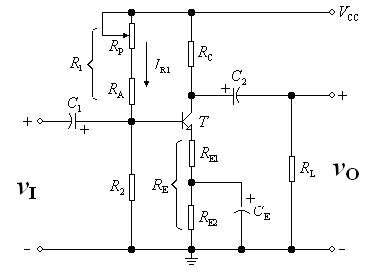
\includegraphics{pic/共射放大器.jpg}
                \caption{电路原理图}
            \end{figure}
        通过戴维南等效可以计算:
        $$V_{BB}=V_{CC}\frac{R_2}{R_1+R_2}$$
        $$R_{BB}=R_1||R_2$$
        $$I_E=\frac{V_{BB}-V_{BE}}{R_E+R_{BB}/(1+\beta)}$$
        $$I_C=\frac{\beta}{1+\beta}I_E \approx I_E$$
        $$V_{CE}=V_{CC}-(R_C+R_E)I_C$$
        \subsection{交流性能指标计算}
        $$g_m=\frac{I_C}{V_T}$$    
        $$R_{\pi}=\frac{\beta}{g_m}$$    
        $$r_e=\frac{\alpha}{g_m}$$
        $$A_v=\frac{v_o}{v_i}\approx-\frac{R'_C}{R'_E}=-\frac{R_C||R_L}{r_e+R_{E1}}$$
        $$R_i=R_1||R_2||[(1+\beta)(r_e+R_{E1})]$$
        $$R_o\approx R_C$$
    \section{实验方案设计与实验参数计算}
        \subsection{实验方案设计}
        根据性能指标范围确定静态工作点和元件参数值时有一些原则和经验公式可以参照。
            \begin{enumerate}
                \item 在微弱信号放大或前置放大器设计时需要考虑晶体管的噪声系数。通常,高频小信号晶体管工作电流在$0.5mA~2mA$时噪声最小,一般设定在$1mA$以下。
                \item 由静态电流$I_E$,要使静态工作点较稳定,应取$VBB>>VBE$。对硅晶体管,一般取$VBB$为$3V~5V$。
                \item 要保证VB足够稳定,应使$I_{R1}>>I_B$,常取$I_{R1}$为$(5\sim 10)I_B$。
                \item 为获得较大的输出信号摆幅和电压增益,基极静态电压不能太高,工程设计中一般取$V_B$或$V_{BB} \approx (\frac{1}{3}\sim \frac{1}{4})V_{CC}$。
                \item 由于射极电阻$R_{E1}$的负反馈作用,增大$R_{E1}$能提高电路的输入电阻、能提高电压增益的稳定性,但将使电压增益值$|A|_v$下降。另一方面,当电压增益要求给定时,增大$R_{E1}$就需要提高集电极电阻RC,而这将降低晶体管的集电极静态电压$V_C$、影响输出信号摆幅。因此,$R_{E1}$、$R_C$的确定需要根据电压增益$|A|_v$的大小及稳定性、输入电阻要求、输出信号摆幅等进行综合考虑。
                \item 耦合电容$C_1$、$C_2$和旁路电容$C_E$的取值。一般来说,$C_1$、$C_2$、$C_E$取值越大,放大器的下限截止频率越低。但电容越大,体积也大、漏电电流也大。如果放大器的低频特性要求不是很苛刻,没有必要每次都计算这三个电容值。$C_1$、$C_2$常取$(10\sim 20)μF$、$C_E$常取$(30\sim 100)μF$。
            \end{enumerate}
        \subsection{实验参数计算}
        \begin{enumerate}    
            \item 实验参数:
                \begin{enumerate}
                    \item 我对实验给定的实验参数进行了些调整如下:\\$V_{CC} = +15V,\, R_L = 4.7k \Omega ,\,  V_i = 10mV,\, R_s = 600 \Omega$
                    \item 考虑到晶体管的噪声系数,取$I_C = 0.8mA$
                    \item 为了使静态工作点较稳定同时获得较打的输出信号摆幅和电压增益,取$V_{BB} = 3.92V$
                    \item 为了满足上述条件,同时考虑到电阻的标称值,取$R_1 = 110k \Omega ,\, R_2 = 39k \Omega$
                    \item 根据电压增益的大小以及稳定性、输入电阻的要求综合考虑,取$R_{E1} = 56 \Omega ,\, R_{E2} = 3.6k \Omega ,\, R_C = 3.6k \Omega $
                \end{enumerate}
            \item 结果计算:\par
            根据实验原理所示公式,计算具体结果如下:\\
            $$V_{BB}=V_{CC}\frac{R_2}{R_1+R_2} = 3.93V$$
            $$I_E=\frac{V_{BB}-V_{BE}}{R_E+R_{BB}/(1+\beta)} = 0.84mA$$
            $$I_C=\frac{\beta}{1+\beta}I_E \approx I_E = 0.84mA$$
            $$V_{CE}=V_{CC}-(R_C+R_E)I_C = 8.90V$$
            $$A_v=\frac{v_o}{v_i}\approx-\frac{R'_C}{R'_E}=-\frac{R_C||R_L}{r_e+R_{E1}} = -23.51 V/V$$
            $$R_i=R_1||R_2||[(1+\beta)(r_e+R_{E1})] = 9.401k  \Omega $$
            $$R_o\approx R_C = 3.6k \Omega $$
        \end{enumerate} 
    \section{主要仪器设备}
        电路、示波器、信号发生器、万用表、电阻若干、电容若干、电源
    \section{实验仿真}
        \subsection{测量$I_C$、$V_{CE}$}
            \begin{enumerate}
                \item 利用Bias Point仿真分析
                    \begin{figure}[h]
                        \centering
                        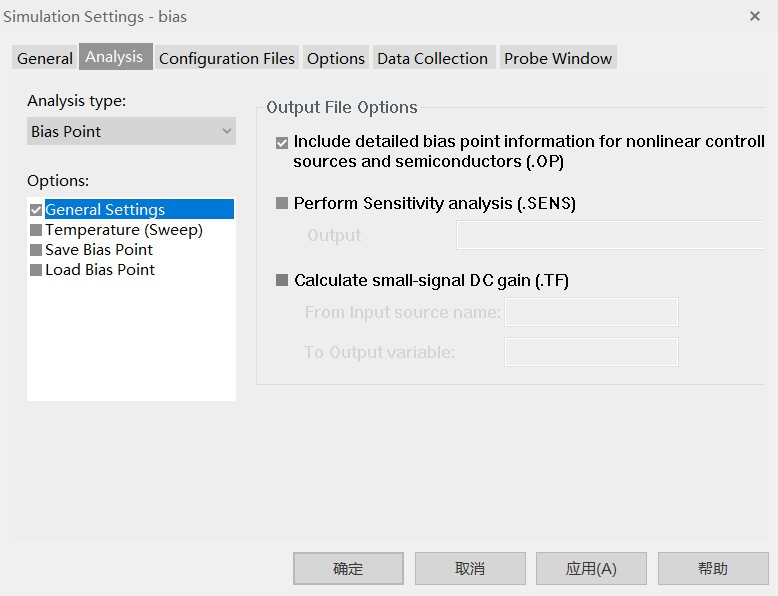
\includegraphics[scale = 0.6]{pic/仿真1}
                        \caption{测量$I_C$、$V_{CE}$}
                    \end{figure}
                \item 在输出结果中查看结果
                    \newpage
                    \begin{figure}[h]
                        \centering
                        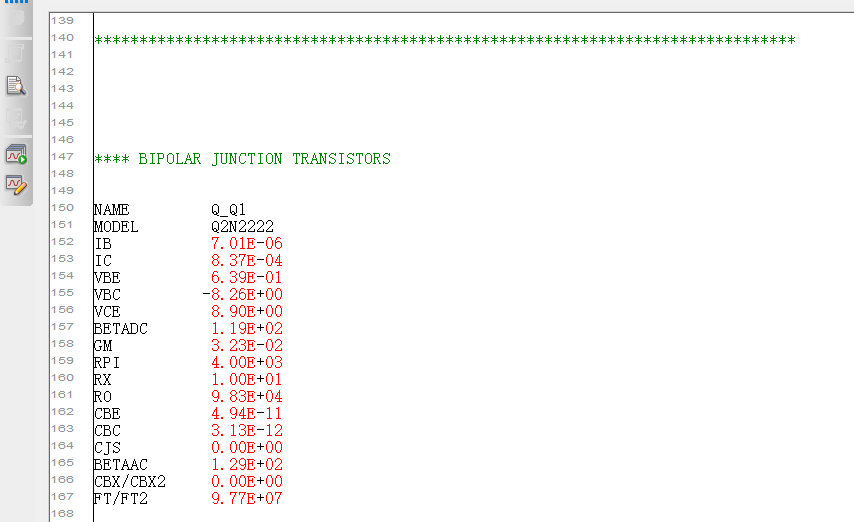
\includegraphics[scale = 0.8]{pic/结果1}
                        \caption{结果}
                    \end{figure}
                    得到:
                    $$I_C = 0.837mA,\, V_{CE} = 8.9V$$
            \end{enumerate}
        \subsection{测量$A_V$、$f_L$、$f_H$}
        \begin{enumerate}
            \item 利用AC Sweep/Noise仿真分析
                \newpage
                \begin{figure}[h]
                    \centering
                    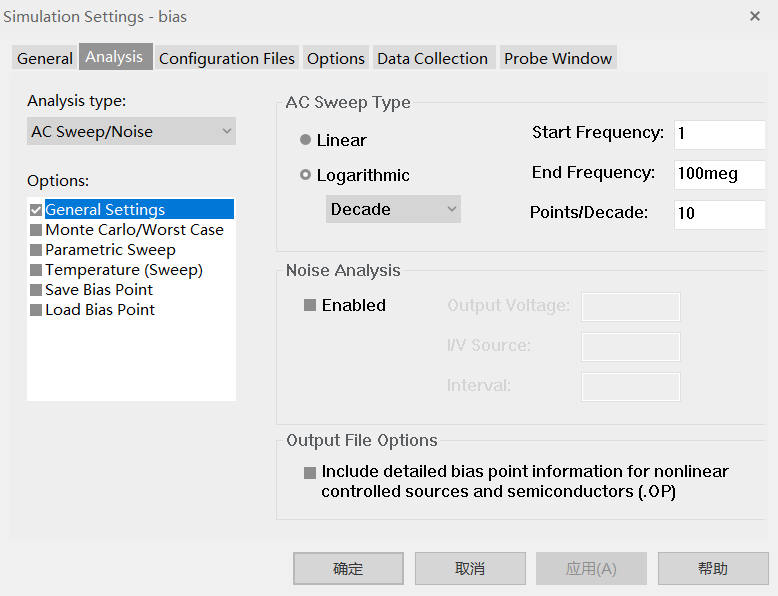
\includegraphics[scale = 0.6]{pic/仿真2}
                    \caption{仿真设置}
                \end{figure}
                \begin{figure}[h]
                    \centering
                    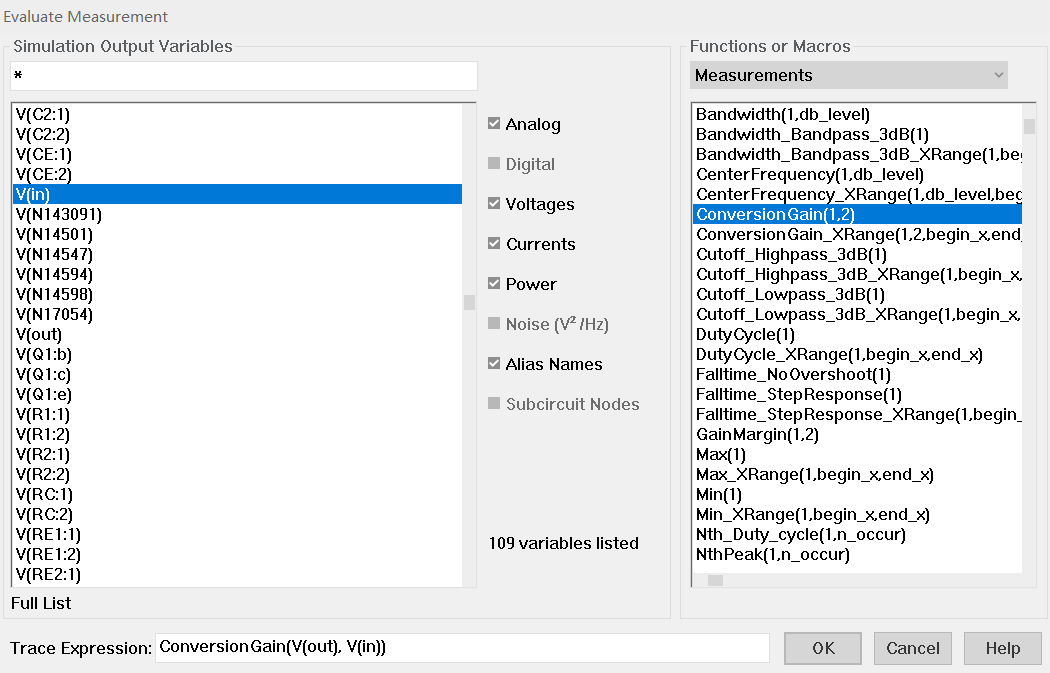
\includegraphics[scale = 0.5]{pic/仿真3}
                    \caption{仿真设置}
                \end{figure}
            \item 在输出结果中查看结果
                \newpage
                \begin{figure}[h]
                    \centering
                    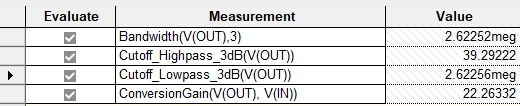
\includegraphics[scale = 1]{pic/结果2}
                    \caption{结果}
                \end{figure}
                得到:
                $$A_V = -22.26,\, f_H  = 39.29Hz,\, f_L = 262.26kHz$$
        \end{enumerate}
        \subsection{测量$R_i$、$R_o$}
            \subsubsection{测量$R_i$}
            \begin{enumerate}
                \item 利用AC Sweep/Noise仿真分析
                    % \newpage
                    \begin{figure}[h]
                        \centering
                        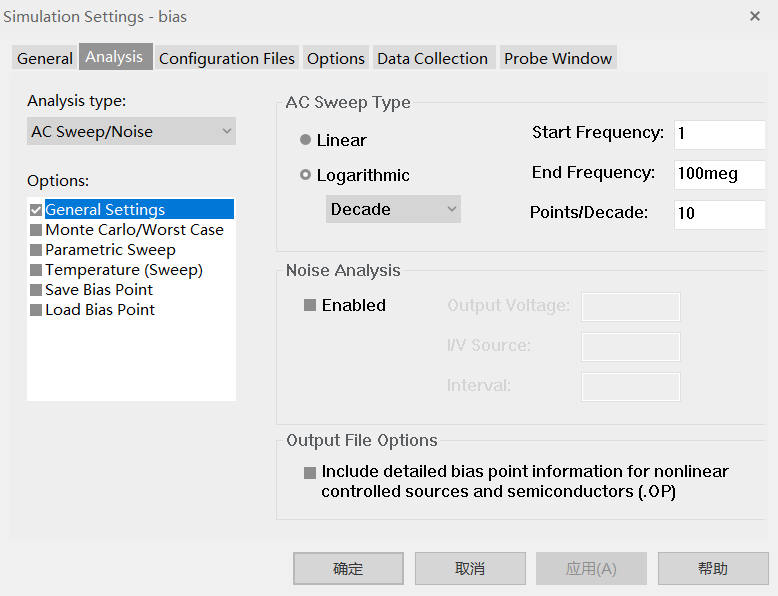
\includegraphics[scale = 0.6]{pic/仿真2}
                        \caption{仿真设置}
                    \end{figure}
                    \begin{figure}[h]
                        \centering
                        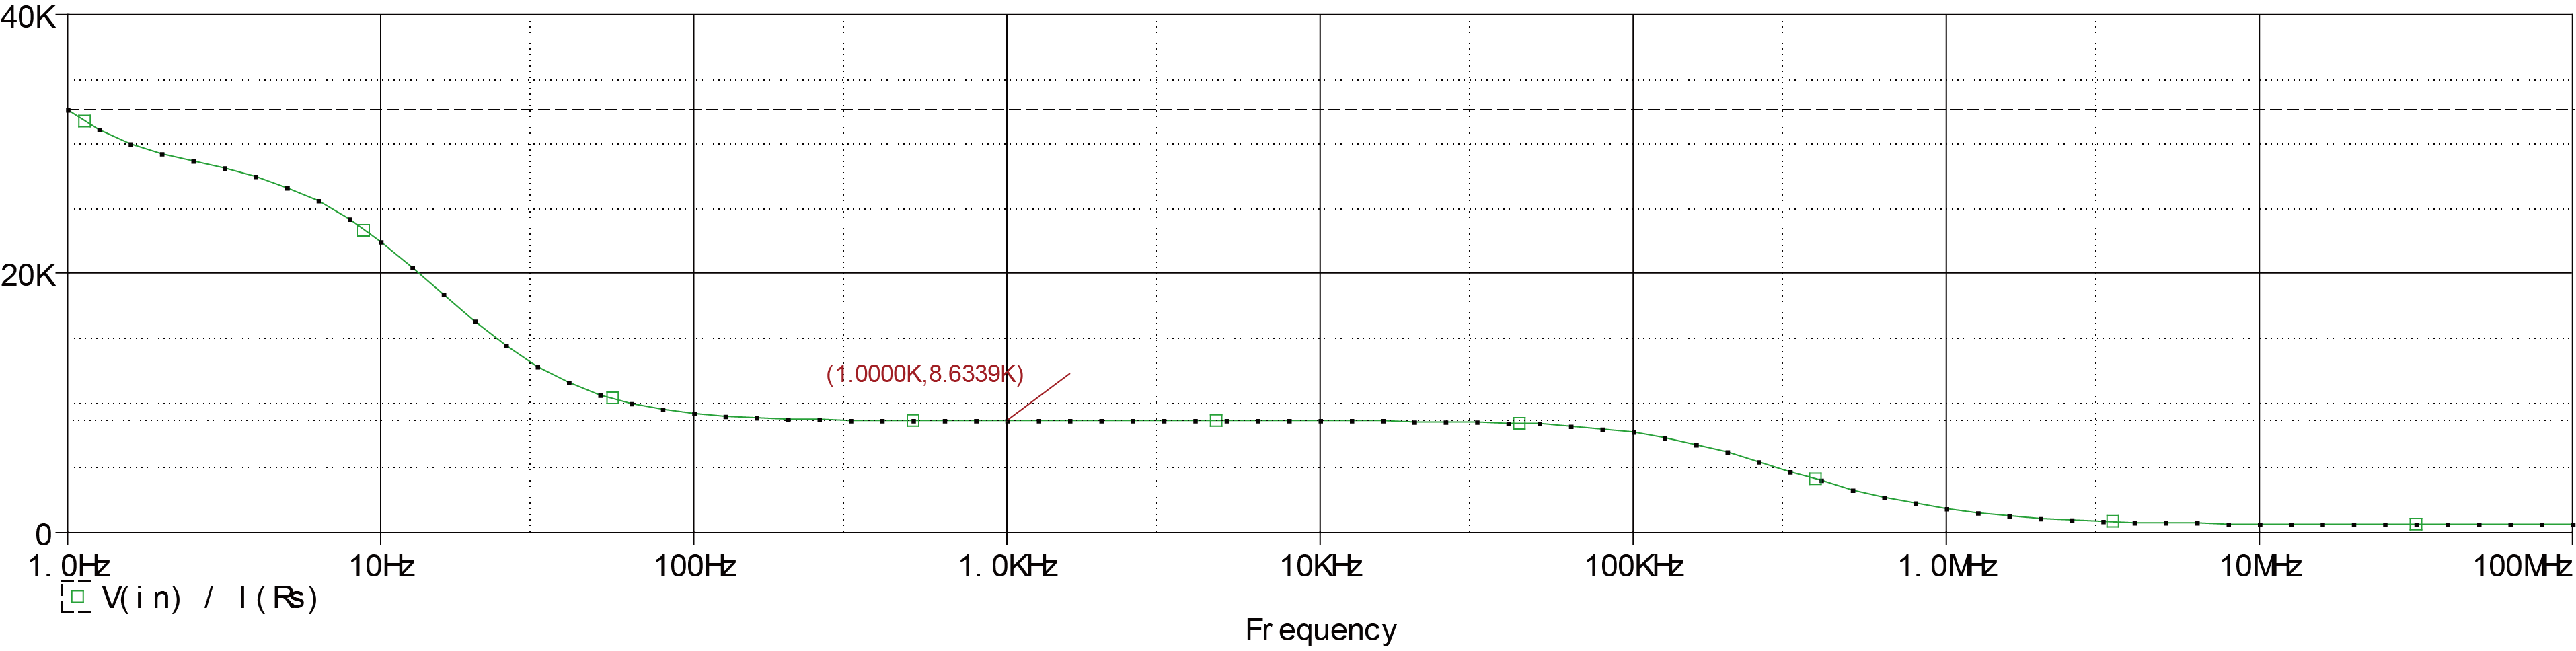
\includegraphics[scale = 0.4]{pic/ri}
                        \caption{结果}
                    \end{figure}
                    得到:
                    $$R_i = 8.6339k\Omega$$
            \end{enumerate}
            \subsubsection{测量$R_o$}
            \begin{enumerate}
                \item 更改电路图如下图
                    % \newpage
                    \begin{figure}[h]
                        \centering
                        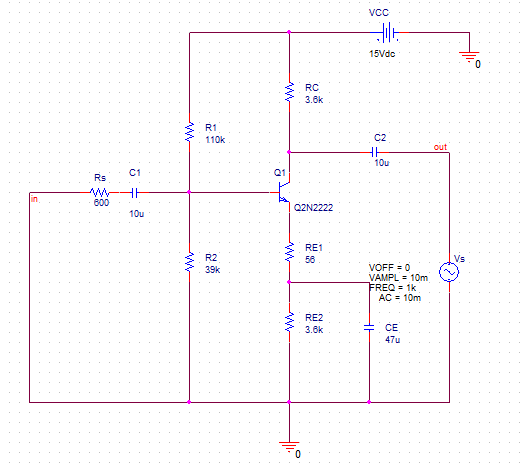
\includegraphics[scale = 0.8]{pic/仿真4}
                        \caption{电路图}
                    \end{figure}
                \item 利用AC Sweep/Noise仿真分析
                    \newpage
                    \begin{figure}[h]
                        \centering
                        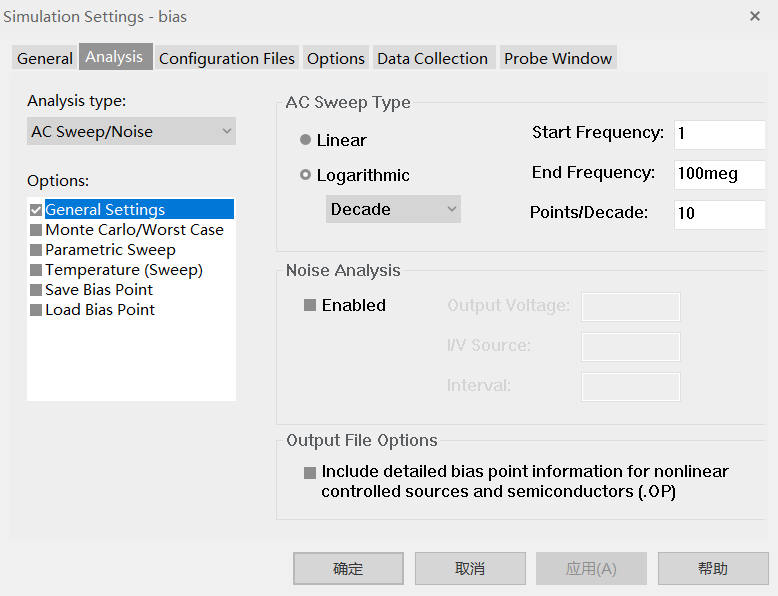
\includegraphics[scale = 0.6]{pic/仿真2}
                        \caption{仿真设置}
                    \end{figure}
                    \begin{figure}[h]
                        \centering
                        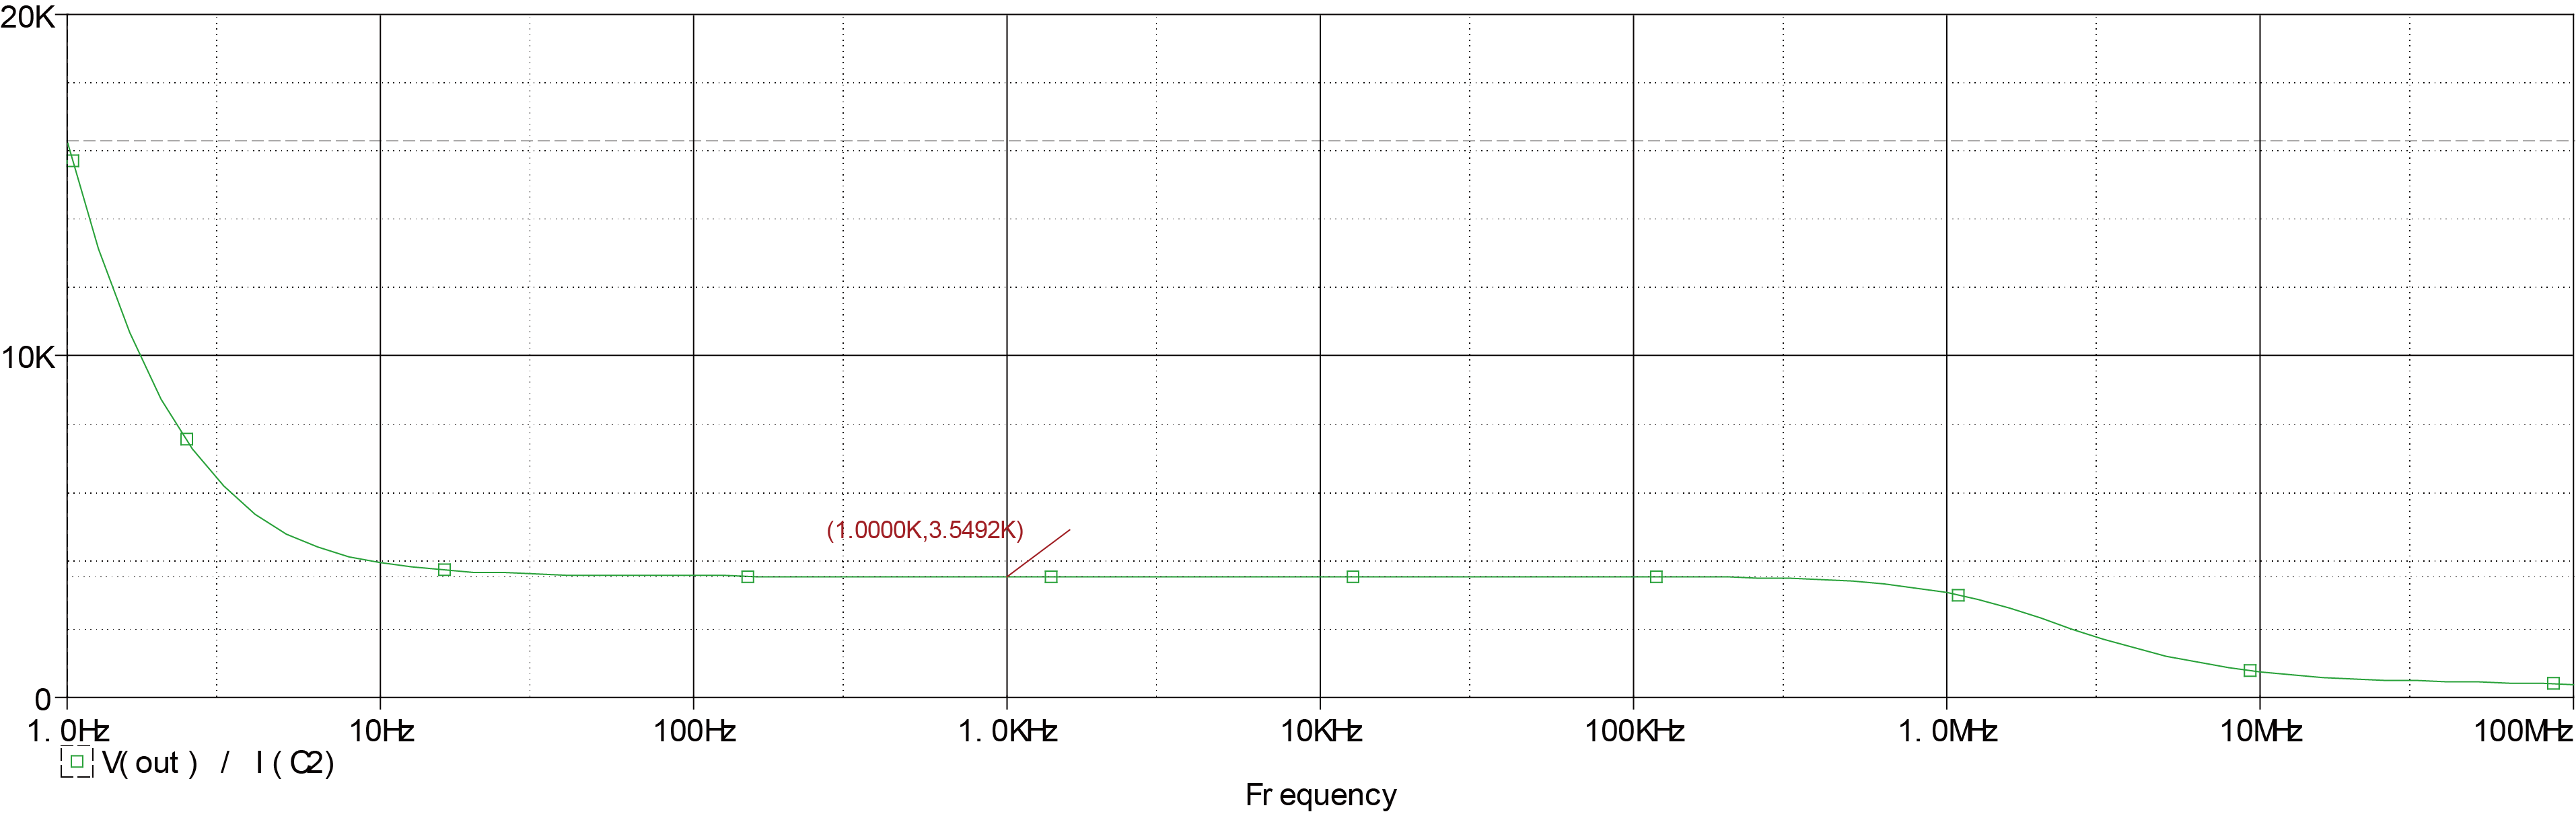
\includegraphics[scale = 0.4]{pic/ro}
                        \caption{结果}
                    \end{figure}
                    得到:
                    $$R_o = 3.5492k\Omega$$
            \end{enumerate}
    \section{实验步骤、实验调试过程、实验数据记录}
        \subsection{实验参数}
        实验中采用了小组组员的参数,如下:
        $V_{CC} = +12V,\, R_L = 5.1k\Omega,\, v_i = 12mV,\, R_1 = 117k\Omega,\, R_2 = 39k\Omega,\, R_C = 3.3k\Omega,\, R_{E1} = 62\Omega,\, R_{E2} = 3.6k\Omega$
        \subsection{实验电路}
            \begin{figure}[h]
                \centering
                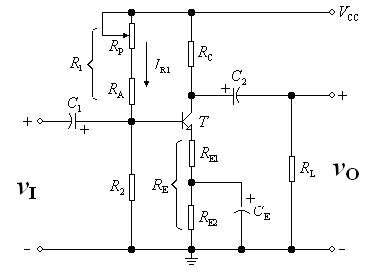
\includegraphics{pic/共射放大器.jpg}
                \caption{实验电路}
            \end{figure}
        \subsection{静态工作点调整与测量}
            \begin{enumerate}
            \item 按元器件参数安装、连接电路。
            \item 不加输入信号。调节$R_P$(板上$R_{W1}$),使$I_C$为设计值(测量电阻$R_C$两端的压降$V_{Rc}$)。
            \item 测量放大电路的静态工作点,并将理论估算值与测量值记录在下表中。
            \end{enumerate}
            \begin{table}[htbp]
                \centering
                \begin{tabular}{|c|c|c|c|c|}
                \hline
                $mA$、$V$ & $I_C$ &  $V_{CE}$& $V_{BE}$ & $V_B$ \\ \hline
                 理论估计& 0.728 & 8.93 & 0.7 & 3.5 \\ \hline
                 测量& 0.729 & 8.90 & 0.61 & 3.58 \\ \hline
                \end{tabular}
                \caption{静态工作点调整与测量}
            \end{table}
            \subsection{电压增益测量}
            \begin{enumerate}
                \item 保持$I_C$不变,调节信号源,使输出$1kHz$正弦波,加至放大电路输入端,使输入电压$v_i$幅度$30mV$(以示波器显示为准)
                不接负载电阻,即:$R_L = \infty $(开路)。
                输入、输出波形用双踪显示观察,指出它们的相位关系。
                当输出波形无失真时,分别读出$v_i$ 、$v_o$的峰-峰值,记入下表。
                \item 增大输入信号幅度,用示波器监视输出波形。使输出波形出现失真,记下此时输出波形草图,说明首先出现的是哪种失真。测出最大不失真输出电压峰-峰值,记入下表。
                \\
                \newpage
                \begin{figure}[h]
                    \centering
                    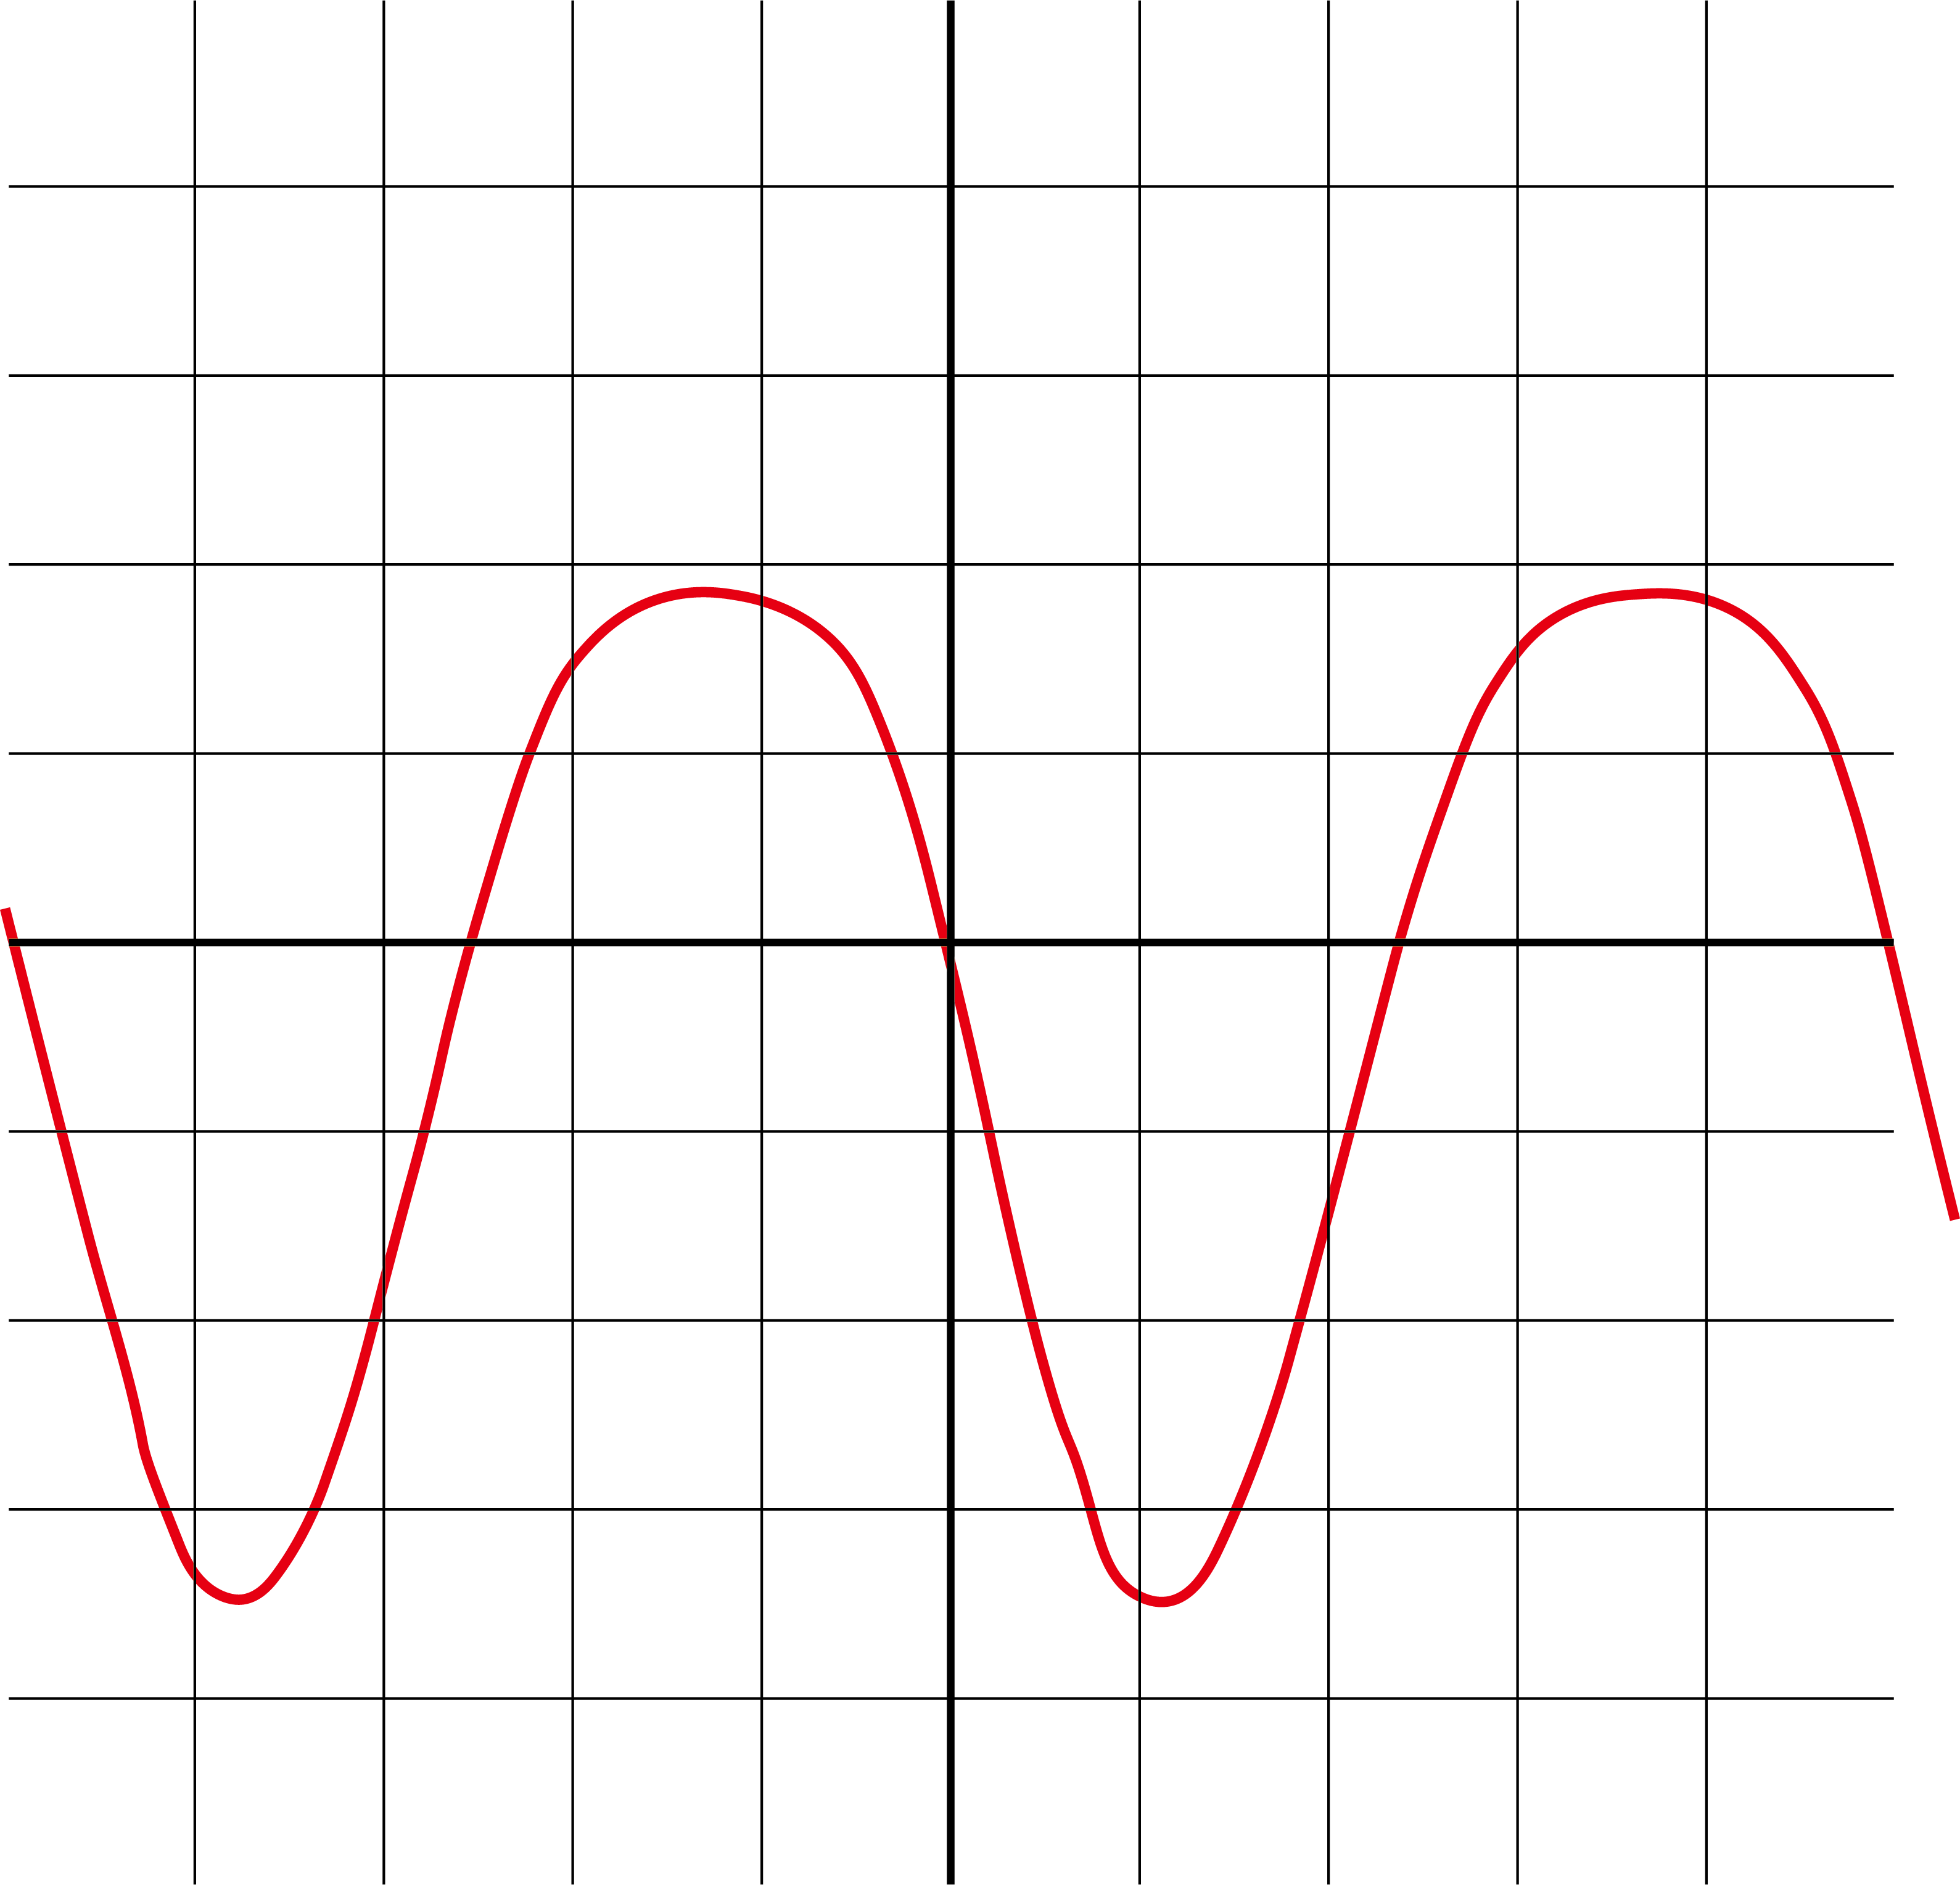
\includegraphics[scale = 0.2]{pic/草图}
                    \caption{波形图草图}
                \end{figure}
                结果:首先出现的是截止失真。
                \item 入负载 $R_L= 5.1k\Omega$。重做步骤(1),记入表中。
                计算电压增益 $A_V$ ,分析负载对电压增益的影响。              
                \begin{table}[h]
                    \centering
                    \begin{tabular}{|c|c|c|c|c|c|}
                    \hline
                    \multirow{2}{*}{测试条件} & \multicolumn{4}{c|}{实测值(峰-峰值)} & 理论值 \\ \cline{2-6} 
                                        &   $V_i$  &  $V_o$   &  $V_omax$   &  $A_V$   & $A_V$ \\ \hline
                                        $R_L = \infty$  &  $60mV$   &  $2V$   &  $2.2V$   &  -33.33   & -33.86 \\ \hline
                                        $R_L = 5.1k \Omega $  &  $60mV$   &  $1.192V$   &  $\times$   &   -19.87  & -20.56 \\ \hline
                    \end{tabular}
                    \caption{电压增益测量}
                \end{table}
            \end{enumerate}
            \subsection{输入电阻输出电阻测量}
                \subsubsection{输入电阻测量}
                在信号源与被测放大器之间串入一个与 $R_i$ 同一数量级(理论估算)的已知电阻 $R$ ,在输出波形不失真的情况下,分别测出 $v_s$ 和 $v_i$ ,则放大器的输入电阻为
                $$R_i = \frac{v_i}{(v_s - v_i)/R} = \frac{v_i}{v_s - v_i} \times R $$
                \begin{table}[h]
                    \centering
                    \begin{tabular}{|c|c|c|c|c|}
                    \hline
                    $R_i$(理)        & $R$   & $v_s$    & $v_i$  & $R_i$(实) \\ \hline
                    $1.0213k\Omega$ & $10k\Omega$ & $30.2mV$ & $15mV$ & $9.868k\Omega$ \\ \hline
                    \end{tabular}
                    \caption{输入电阻测量}
                \end{table}
            \subsubsection{输出电阻测量}
            输出波形不失真情况下,分别测出输出端空载时的输出电压 $v_o$、和接入负载 $R_L$ 后的输出电压 $v_o’$,则放大器的输出电阻为
            $$R_o = \frac{v_o - v_o'}{v_o'/R_L} = (\frac{v_o}{v_o'}-1)\times R_L$$
            \begin{table}[h]
                \centering
                \begin{tabular}{|c|c|c|c|}
                \hline
                $v_o$           & $v_o'$ & $R_o$(理) & $R_o$  \\ \hline
                $0.416V$ & $0.256V$  & $3.3k\Omega$ & $3.1875k\Omega$ \\ \hline
                \end{tabular}
                \caption{输出电阻测量}
            \end{table}
            \subsection{上限截止频率$f_H$,下限截止频率$f_L$测量}
            电压增益下降到中频增益0.707倍时(分贝数下降3dB)所对应的上、下限频率即 $f_H$、$f_L$。\\
            放大电路的通频带宽度$B_W$。即 $B_W = f_H - f_L$ \par
            测量方法
                \begin{enumerate}
                \item 在$I_C$为设计值、$R_L = \infty$情况下,输入	$1kHz$正弦信号,改变输入信号幅度,使输出电压峰-峰值为	$0.5V{OP-Pmax}$左右(主要是为了避免输出过大而出现失真或输出过小影响测量精度)。准确测出此时输出电压峰-峰值$VOp-p$。
                \item 保持放大器输入电压$v_i$幅度不变,改变信号源输出频率(增加	或减小),当输出电压值达到$0.707V{Op-p}$值时,停止信号源	频率的改变,此时信号源所对应的输出频率即为 $f_H$ 、或 $f_L$。\\
                测得:\\
                $$V_{Op-p} = 1.104V$$
                $$f_H = 37.0Hz$$
                $$f_L = 275kHz$$
                \end{enumerate}
    \section{实验结果与分析}
    最后的实验是采用的组员的设计参数,如下\\
    $V_{CC} = +12V,\, R_L = 5.1k\Omega,\, v_i = 12mV,\, R_1 = 117k\Omega,\, R_2 = 39k\Omega,\, R_C = 3.3k\Omega,\, R_{E1} = 62\Omega,\, R_{E2} = 3.6k\Omega$
    \begin{table}[h]
        \centering
        \begin{tabular}{|c|c|c|c|c|c|c|c|}
        \hline
            & $I_C$     & $V_{CE}$  & $A_V$     & $R_i$           & $R_o$           & $f_L$      & $f_H$       \\ \hline
        理论值 & $0.728mA$ & $8.9283V$ & $-20.556$ & $1.0213k\Omega$ & $3.3k\Omega$    & $34.51Hz$  & $\times$    \\ \hline
        仿真  & $0.7271mA$ & $8.915V$  & $-20.261$ & $8.7118k\Omega$ & $3.2649k\Omega$ & $37.115Hz$ & $224.46kHz$ \\ \hline
        测量  & $0.729mA$   & $8.90V$    & $-19.87$  & $9.868k\Omega$  & $3.1875k\Omega$ & $37.0Hz$   & $275kHz$    \\ \hline
        \end{tabular}
        \caption{结果比较}
        \end{table}
        从结果中可以看出,测量值和仿真、设计值比较符合,同时也满足最初的设计要求。同时由于仿真软件中三极管与设计和实验中的三极管有所区别导致最后$R_i$相对误差偏大。
    \section{讨论、心得}
    以前在电子电路基础的课程学习的时候,仅仅是简单的从理论层面对该放大电路进行分析,并没有真正理解电路中每个元件的作用以及每个元件的大小取舍会怎样影响放大效果。但是通过本次实验,我学会了如何根据设计要求去选择每个元件,知道了每个电阻和电容的大小会怎样影响电路的放大效果。
    其次,通过本次实验,我对OrCAD软件的使用有了更加深入的理解,认识到其的强大,但是也了解到了仿真可能带来的误差。
\end{document}